\documentclass{article} % For LaTeX2e
\usepackage{iclr2016_conference,times}
\usepackage{hyperref,algorithm,algpseudocode,array,tabularx,multirow,caption,subcaption,amsfonts,url,verbatim,enumitem,amsmath,graphicx}
\usepackage{url}

\title{Fast Parallel SAME Gibbs Sampling on \\ General Discrete Bayesian Networks}

\author{Daniel Seita, Haoyu Chen \& John Canny \\
Computer Science Division \\
University of California, Berkeley \\
Berkeley, CA 94720, USA \\
\texttt{\{seita,haoyuchen,canny\}@berkeley.edu}
}

% The \author macro works with any number of authors. There are two commands used to separate the
% names and addresses of multiple authors: \And and \AND.
%
% Using \And between authors leaves it to \LaTeX{} to determine where to break the lines. Using \AND
% forces a linebreak at that point. So, if \LaTeX{} puts 3 of 4 authors names on the first line, and
% the last on the second line, try using \AND instead of \And before the third author name.
%
% ICLR requires electronic submissions, processed by \url{http://arxiv.org}. See ICLR's website for
% more instructions.
% 
% If your paper is ultimately accepted, the statement {\tt {\textbackslash}iclrfinalcopy} should be
% inserted to adjust the format to the camera ready requirements.
% 
% The format for the submissions is a variant of the NIPS format.  Please read carefully the
% instructions below, and follow them faithfully.

\newcommand{\fix}{\marginpar{FIX}}
\newcommand{\new}{\marginpar{NEW}}

%\iclrfinalcopy % Uncomment for camera-ready version

\begin{document}

\maketitle

\begin{abstract}
A fundamental task in machine learning and related fields is to perform inference on Bayesian
networks. Since exact inference takes exponential time, it is common to use an approximate algorithm
such as Gibbs sampling, but this can still be intractable for graphical models with hundreds of
binary random variables. In this paper, we address this issue by presenting our highly optimized
Gibbs sampler, which we believe is the fastest one publicly available.  Our Gibbs sampler is
GPU-accelerated, heavily parallelized, and replicates data via State Augmented Marginal Estimation
(SAME) to decrease convergence time while reaching higher quality parameter estimates.  Experiments
on both synthetic and real data show that our Gibbs sampler is substantially faster than the state
of the art sampler, JAGS, without sacrificing accuracy. Our ultimate objective is to introduce the
Gibbs sampler to researchers in many fields to expand their range of feasible inference problems.
\end{abstract}




\section{Introduction}\label{sec:intro}

In many machine learning applications, the user has a distribution $P(X,Z \mid \Theta)$ where $X$ is
observed data, $Z$ is hidden (latent) data, and $\Theta$ represents the model parameters. The goal
is generally to find an optimal $\Theta$ with respect to $X$, while marginalizing out $Z$. To
represent these problems, it is common to use graphical models, which combine probability theory and
graph theory to present a robust formalism for probabilistic inference. A Bayesian network is a
graphical model defined by a directed acyclic graph and a set of conditional probability tables
(CPTs). Each CPT represents a local probability distribution $\Pr(X_i \mid X_{\pi_i})$ where $X_i$
is a random variable, and $X_{\pi_i}$ represents its set of parent nodes in the graph. We denote the
full set of CPTs as $\Theta$.

In this paper, our focus is on parameter estimation of Bayesian networks with discrete random
variables (``discrete Bayesian networks'') based on partially observed data $\mathcal{D} = \{\xi_1,
\ldots, \xi_m\}$, where $\xi_i$ is an $n$-dimensional vector with assignments to the $n$ variables
of the graph, or ``N/A'' to indicate missing data. We assume that the structure of the Bayesian
network --- its nodes and edges --- is known in advance. This type of problem often arises in
practice because it is easier to elicit graph structure from human experts than it is to get
numerical parameters~\citep{Koller2009}. Furthermore, it is often unrealistic to expect our data
$\mathcal{D}$ to be completely observed, as data might be missing due to errors (e.g., human
oversights) or deliberate omissions.

Well-known strategies for parameter estimation with partially observed data include
Expectation-Maximization~\citep{EMpaper} and variations of gradient ascent~\citep{Thiesson95}.
Parameter estimation using these methods requires running probabilistic inference over the missing
data, which tends to be the limiting factor since  exact inference using the junction tree algorithm
takes exponential time. It is therefore common to use approximate inference procedures.  One way is
to perform Markov Chain Monte Carlo (MCMC) simulation, where one constructs a Markov chain whose
states are an assignment to all unobserved variables, such that the stationary distribution of the
chain is the posterior probability over these variables.

Gibbs sampling~\citep{Geman1984} is a special case of MCMC simulation, which at iteration $t$, goes
through each unobserved variable and samples from its full conditional based on the samples from the
current or previous iteration: $X_i^{(t)}\ {\raise.17ex\hbox{$\scriptstyle\sim$}} \
\Pr(X_i^{(t)} \mid X_1^{(t)}, \ldots, X_{i-1}^{(t)}, X_{i+1}^{(t-1)}, \ldots, X_n^{(t-1)})$. For the
parameter estimation problem, one also needs to sample to update $\Theta$ from $P(\Theta
\mid \mathcal{D})$, the posterior distribution over the complete data data $\mathcal{D}$
(``complete'' due to sampling). Since we assume discrete random variables, the samples are
multinomial counts, so for Bayesian estimation, one can impose a set of Dirichlet priors on
$\Theta$ so that the posterior is also a set of Dirichlets.

While Gibbs sampling is commonly used in machine learning, it is a very broad technique that may not
be able to match the performance of special-purpose inference algorithms without extensive
fine-tuning or using complicated variations~\citep{Murphy2012}. \textbf{Daniel: I am not sure if I
am explaining this last sentence well enough. Murphy's book has some explanation, but not much.} In
a recent result,~\citet{SAME2015} showed that by combining the State Augmented Monte Carlo (SAME)
technique~\citep{SAME2002} with Gibbs sampling, one can get fast, high quality parameter estimates
for discrete graphical models, but they only applied it to two specific models that do not have
mutual dependencies between discrete states.  In this paper, we build upon that result by
presenting a SAME Gibbs sampler for general discrete Bayesian networks. To be precise, the
novelty and aspects of our Gibbs sampler is that

\begin{itemize}[noitemsep]
    \item our sampler uses an adjustable SAME parameter to replicate data, causing the Gibbs sampler
    to converge faster to higher-quality MAP or ML parameter estimates. We believe this is due to
    reduction of excess variance from standard Gibbs sampling.
    \item we run our sampler on state of the art GPUs and parallelize it as much as possible. Our
    sampler can ultimately scale up to problems with hundreds of random variables.
    \item the sampler is designed to maximize throughput on only one computer, thus avoiding the
    need to work though complicated distributed systems.
    \item it is open source as part of the BIDMach
    library\footnote{\url{https://github.com/BIDData/BIDMach}} and comes with various diagnostic
    tools. Furthermore, BIDMach's mini-batch updating and matrix caching features mean we could even
    run our Gibbs sampler on data too large to fit in a computer's RAM.
\end{itemize}

We benchmark our sampler versus the state of the art Gibbs sampler, JAGS~\citep{JAGS2003}, and show
that our Gibbs sampler is multiple orders of magnitude faster. Consequently, in addition to
introducing our Gibbs sampler to researchers, we argue in this paper that Gibbs sampling augmented
with SAME can be competitive with or superior to the fastest special purpose inference algorithms
for Bayesian inference. \textbf{Daniel: my main concern is that we are not talking about these
``special purpose inference algorithms.'' We're presenting a fast SAME Gibbs sampler, and I don't
know a good way to incorporate factor graphs~\citep{Factorie2009}.}





\section{Related Work}\label{sec:related_work}

The problem of Bayesian inference for graphical models is old and well-studied, and for reference,
we refer the reader to textbooks (e.g., see~\citet{Koller2009} for a broad background) and survey
papers (e.g., see~\citet{Wainwright2008} for a discussion on variational inference as an alternative
to MCMC methods). \textbf{Daniel: I would like to have a survey paper that actually compares Gibbs
sampling versus other methods. I think this paragraph should be expanded, while condensing the
introductory section.}

Gibbs sampling is also relatively old and well-studied, but it has recently been getting more
attention as the research community explores efforts to improve speed and scalability. The Gibbs
sampling research most related to our contribution involves efforts to (1) parallelize Gibbs
sampling and (2) achieve high throughput. By exploiting the conditional independence assumptions of
Bayesian networks, is possible to have an exact, semi-parallel Gibbs sampler that iterates through
color groups of nodes, and within each group, sampling each node independently~\citep{Gonzalez2011},
a strategy that we employ in our sampler. It is also possible to relax the sequential nature of the
algorithm and approximate Gibbs sampling by limiting global communication~\citep{Johnson2013}.  The
databases community has also been able to contribute to speeding up Gibbs sampling by showing how
improved system design can lead to higher throughput~\citep{Zhang2013}.

Recently, the use of Graphics Processing Units (GPUs) has become essential for developing high
performance software, as exemplified by popular packages such as Theano for evaluating mathematical
expressions with multidimensional arrays~\citep{Theano2012} and CAFFE for neural
networks~\citep{jia2014caffe}.  The Augur probabilistic programming language~\citep{Augur2014},
which generates inference code for Bayesian networks, demonstrates the importance of combining GPU
code with extra parallelism introduced from exploiting conditional independence assumptions.

The result most directly related to our paper, as briefly mentioned in Section~\ref{sec:intro}, is
one that shows how the addition of SAME to a GPU-accelerated Gibbs sampler can be very fast for
Latent Dirichlet Allocation and the Chinese Restaurant Process~\citep{SAME2015}. In that paper, they
explored the application of SAME to graphical model inference on modern hardware, and showed that
combining SAME with factored sample representation (or approximation) gives throughput competitive
with the fastest symbolic methods, but with potentially better quality. We (non-trivially) extend
their result by implementing a general-purpose Gibbs sampler that can be applied to arbitrary
discrete graphical models.





\section{Fast Parallel SAME Gibbs Sampling}\label{sec:same}

SAME is a variant of MCMC where one artificially replicates data to create distributions that
concentrate themselves on the global modes~\citep{SAME2002}. It is an efficient way of performing
MAP estimation in high-dimensional spaces when needing to integrate out a large number of variables.
Given a distribution $P(X,Z\mid \Theta)$, to estimate the most likely $\Theta$ based on the data
$(X,Z)$ using SAME, one would define a new joint $Q$:
\begin{equation}\label{eq:same}
Q(X,\Theta,Z^{(1)},\ldots,Z^{(m)}) = \prod_{j=1}^m P(X,\Theta,Z^{(j)})
\end{equation}
which models $m$ copies of the distribution tied to the same set of parameters $\Theta$, which in
our case forms the set of Bayesian network CPTs. This new distribution $Q$ is proportional to a
\emph{power} of the original distribution, so $Q(\Theta \mid X) \propto (P(\Theta \mid X))^m$. Thus,
it has the same optima, including the global optimum, but its peaks are sharpened~\citep{SAME2002}.
Note that as $m$ increases, SAME approaches Expectation-Maximization~\citep{EMpaper} since the
distribution would peak at the value corresponding to the maximum likelihood estimate.

We argue that SAME is beneficial for Gibbs sampling because it helps to reduce excess variance.  It
is important, however, not to set the SAME replication factor $m$ too high, because that might
result in getting trapped in local maxima in the sharpened distribution. An ideal setup might be to
start with a low replication factor and gradually increase it, a technique similar to simulated
annealing for gradient descent, because both involve ``cooling'' the target distribution to sharpen
the peaks.

\textbf{Daniel: I am really confused about what I should include for this section. I feel like this
just repeats a lot of the SAME description. It might be necessary to do that, but do we have an idea
on what we want to discuss?}




\section{Implementation of SAME Gibbs Sampling}\label{sec:implementation}

\begin{figure}[t]
\centering
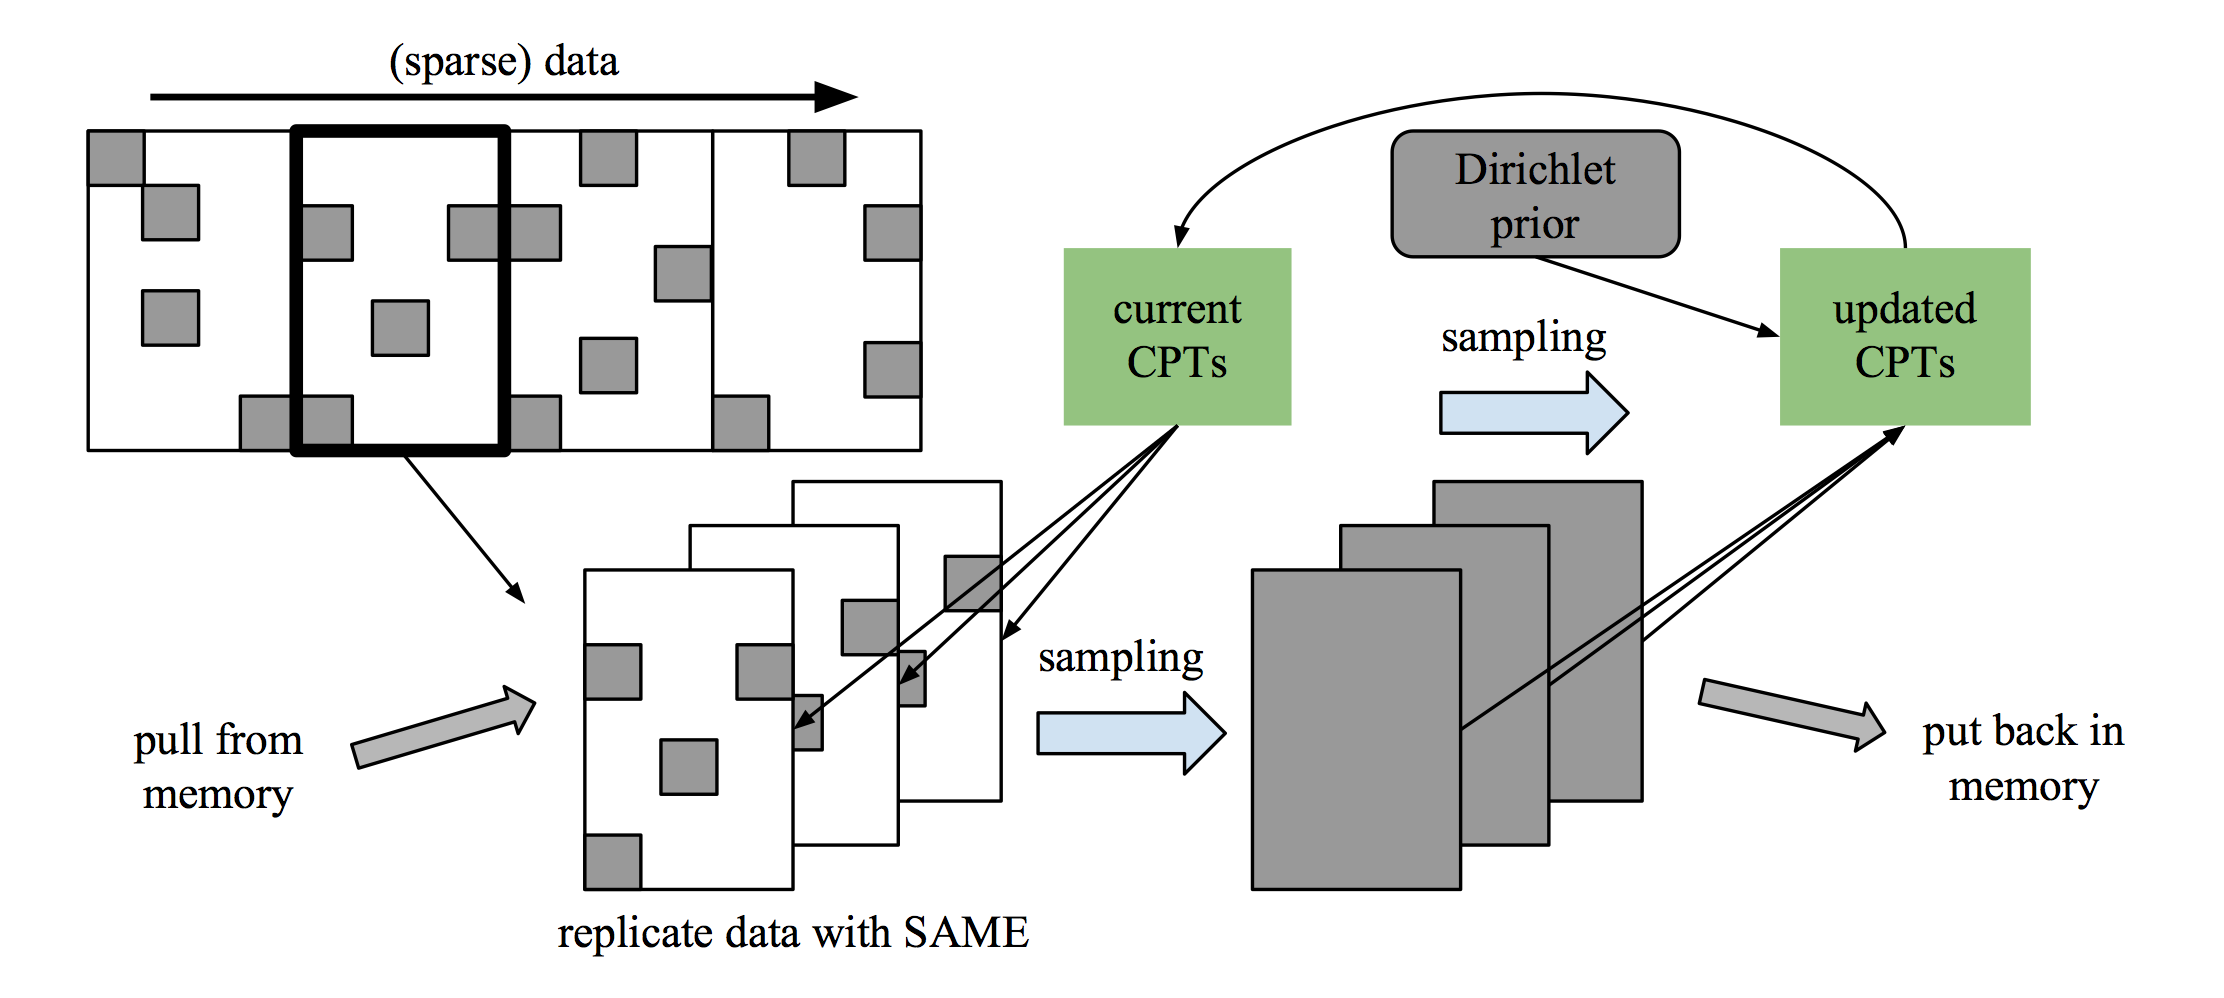
\includegraphics[width=0.8\textwidth]{fig_BIDMach_final}
\caption{This visualizes our Gibbs sampler at work. The original data is split into four
mini-batches of equal sizes (for caching purposes), with each having some known data (shaded gray)
and unknown data (white). For each batch, the sampler replicates the data with SAME $m=3$, samples
the unknown values, then uses those to update the CPTs. The resulting samples are stored in memory
and are used as the starting point for when we sample this batch again.}
\label{fig:BIDMach}
\end{figure}

Our Gibbs sampler is implemented as part of the open-source BIDMach library~\citep{bidmach} for
machine learning.  Figure~\ref{fig:BIDMach} shows a visualization of how it might work on real data.
Our sampler expects a data matrix (typically sparse), with rows representing variables and columns
representing cases. BIDMach divides data into same-sized ``mini-batches'' and iterates through them
to update parameters. Going through all mini-batches is one full pass over the data.

Our Gibbs sampler is augmented with SAME. Consequently, if $m$ is the SAME parameter, for each
mini-batch our sampler forms $m$ copies of the known data.  Then, it performs Gibbs sampling to fill
in the missing data in each copy of the mini-batch using the same set of CPTs.  These sampled
results are combined with an adjustable Dirichlet prior and the current CPTs to form a set of
discrete counts, which are them sampled from to estimate the updated CPTs. To preserve samples
across runs, each time the sampler processes a mini-batch, it stores the sampled results in memory.
Then during the next \emph{pass} over the data, when it reaches this corresponding mini-batch again,
it starts the Gibbs sampling process from that stored data. It is possible to skip the first few
samples (the \emph{burn-in} period) and also to only update the parameters every $N^{\rm th}$
iteration to reduce correlated samples.

There are many ways in which the sampler is optimized to maximize throughput on one computer and to
avoid excess memory allocation. First, it is GPU accelerated and takes advantage of parallelism in
modern hardware by implementing the sampling process using matrix operations. Since memory is scarce
on GPUs (3-12 GB is typical), BIDMach use a matrix caching strategy to reuse memory for matrices of
the same dimensions. This is why the mini-batches need to be of the same size, since the batches and
all other matrices used as part of the sampling computation will be of fixed size. It is possible to
save even more memory by decreasing the number of cases (i.e., columns) per mini-batch. This step is
often necessary if one wishes to use a high SAME parameter.

As mentioned in Section~\ref{sec:related_work}, we further parallelize Gibbs sampling in an
exact manner via chromatic sampling. In Bayesian networks, nodes $u, v \in \mathcal{V}$ are
independent conditioning on a set of variables $\mathcal{C}$ if $\mathcal{C}$ includes at least one
variable on every path connecting $u$ and $v$ in $\tilde{\mathcal{G}}$, which is the \emph{moralized
graph} of the network, which is the graph formed by connecting parents and dropping edge
orientations. That is, vertex set $\mathcal{C}$ separates the dependency between $u$ and $v$.

Suppose there is a $k$-coloring of $\tilde{\mathcal{G}}$ such that each vertex is assigned one of $k$
colors and adjacent vertices have different colors. Denote $\mathcal{V}_c$ the set of variables
assigned color $c$ where $1 \leq c \leq k$. One can sample sequentially from $\mathcal{V}_1$ to
$\mathcal{V}_k$, where within each color group, it samples all the variables in parallel. This
parallel sampler corresponds exactly to the execution of a sequential scan Gibbs sampler for some
permutation over the variables and will converge to the desired distribution because variables
within one color group are independent to each other given all the other variables. Finding the
optimal coloring of a general graph is NP-complete, but efficient heuristics for balanced graph
coloring perform well in many problems.

\textbf{Daniel: TODO Ahhh, I forgot! The stuff in Figure 1 does actually require data to fit in
memory. There are ways we can get around this with more efficient storage but we should make that
explicit, and say that Figure 1 is only for intuition as most data will fit in memory anyway!}




% Daniel: be sure to reference data correctly! Call it "Koller", "Synthetic MOOC", or "Real MOOC".
\section{Experiments}\label{sec:experiments}

We benchmark our Gibbs sampler based on one synthetic and one real dataset. We compare it with
JAGS~\citep{JAGS2003}, which is the most popular and efficient tool for Bayesian inference, and also
uses Gibbs sampling as the primary inference algorithm. We could not find another general-purpose
software package that substantially outperformed JAGS. % I don't think we need to reference BNT.

For all JAGS experiments, we use a single computer with an Intel Core Xeon processor with eight
cores and 2.20 GHz clock speed (E5-2650 Sandy Bridge). The computer has 64 GB of CPU RAM. We also
run our Gibbs sampler on this machine when we evaluate the speed of its CPU version, for the fairest
comparison with JAGS. These benchmarks would be particularly relevant for those who may only want to
use the CPU version of our Gibbs sampler. The CPU version of the sampler does not require or use
GPUs, though the GPU version requires the CPU during initialization.

The GPU and CPU versions are equivalent up to their random number generators (CUDA and Java,
respectively). Therefore, when we are not directly comparing our sampler's CPU speed with JAGS, or
whenever we use its GPU version, we use a different machine with an Intel Core i7 processor with
four cores, 3.40 GHz clock speed, and 16 GB of CPU RAM. Critically, it also has a high-end NVIDIA
GTX Titan X GPU with 12 GB of RAM.  This computer is newer, but its processor is workstation rather
than server grade, and has half the cores compared to our other machine. We observed that the CPU
version of the sampler ran at roughly the same speed on both computers. This implies that the GPU is
primarily responsible for any substantial time differences between the GPU version on the new
machine and the CPU version on the old machine.

We emphasize that the use of single machines in our experiments is deliberate and a strength of our
sampler, as it is cheaper and simpler to run as compared to using a computing cluster.

\subsection{Synthetic ``Koller'' Data}\label{ssec:koller_data}

\begin{figure}[t]
\centering
\begin{subfigure}{.5\textwidth}
  \centering
  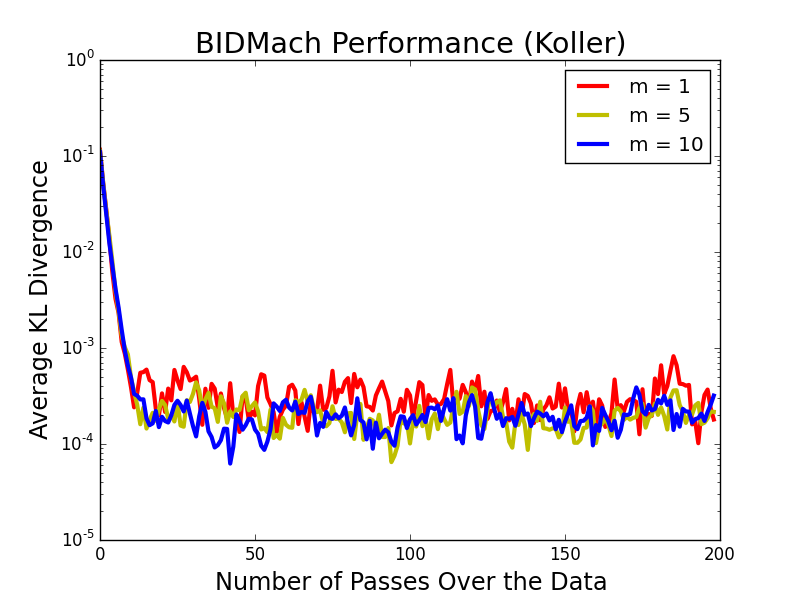
\includegraphics[width=1\linewidth]{fig_kldiv_koller_mb4_gpu}
  \caption{The $KL_{\rm avg}$ from BIDMach.}
  \label{fig:kl_bidmach}
\end{subfigure}%
\begin{subfigure}{.5\textwidth}
  \centering
  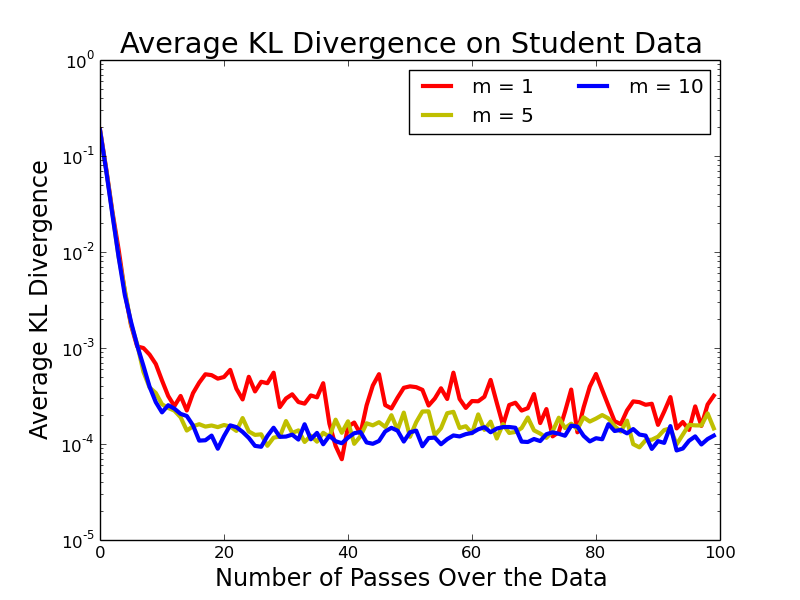
\includegraphics[width=1\linewidth]{fig_kl_div_25_50_perc_jags}
  \caption{The $KL_{\rm avg}$ from JAGS.}
  \label{fig:kl_jags}
\end{subfigure}
\caption{Plots of our $KL_{\rm avg}$ curves as a function of the iteration, on Koller Data. Both
BIDMach and JAGS converge to the true CPTs quickly. (These must be viewed in color.)}
\label{fig:test}
\end{figure}

% BIDMach (CPU) vs JAGS for the Koller data. This one only has 50k columns now!
% BIDMach settings: 25k batch size, 200 iterations, 777 seed.  We do get gflops with BIDMach, so we
% can include them if desired, but the runtime is the more interesting thing we want to compare.
% Perhaps we should use total seconds, rather than per iteration? It's easier to understand.
% Also, opts.updateAll = true because we should be updating after each mini-batch.
%
% Here are the BIDMach CPU (not GPU!) results ON BITTER, with extra values if we can get more JAGS results:
%
% Time=8.7060 secs, gflops=0.84 (m=1)
% Time=15.4930 secs, gflops=0.94 (m=2)
% Time=29.7660 secs, gflops=1.23 (m=5)
% Time=67.6580 secs, gflops=1.08 (m=10)
% Time=129.7780 secs, gflops=1.13 (m=20)
%
% BIDMach CPU times on STOUT, which is what we actually have to report!
%
% Time=10.6480 secs, gflops=0.69 (m=1)
% Time=15.3780 secs, gflops=0.95 (m=2)
% Time=31.4540 secs, gflops=1.16 (m=5)
% Time=61.1170 secs, gflops=1.20 (m=10)
% Time=122.2520 secs, gflops=1.20 (m=20)
%
% Yeah, a  bit weird that gflops doesn't increase each time ... also, funny how stout is actually
% faster. That works to our *advantage* here!
%
% EDIT: Argh, we may have to re-run this to get times for FOUR mini-batches since that's what I use
% for Fig 2. Results on stout with mini-batch sizes of 12.5k:
%
% Time=11.0200 secs, gflops=0.66 (m=1)
% Time=18.0350 secs, gflops=0.81 (m=2)
% Time=33.0970 secs, gflops=1.10 (m=5)
% Time=62.2550 secs, gflops=1.17 (m=10)
% Time=115.3720 secs, gflops=1.27 (m=20)
%
% Make sure we mention in the paper that we're deliberately handicapping ourselves. EDIT: wait, wow,
% 12500 can even be faster in some cases? Yeah, CPU runtime is tricky, but these are ballparks anyway.
\begin{table}[t]
\caption{BIDMach (CPU) vs. JAGS Runtime on Koller Data}
\label{tab:bidmach_jags_koller}
\begin{center}
\begin{tabular}{ |c|c|c|c|c|c|c| } 
\hline
                  & $m=1$ & $m=2$ & $m=5$ & $m=10$ & $m=20$ \\
\hline \hline
BIDMach Time/Iter & 0.055 & 0.090 & 0.165 & 0.311  & 0.577  \\ 
JAGS Time/Iter    & 0.210 & 0.491 & 1.406 & 2.675  & 5.188  \\
\hline
\end{tabular}
\end{center}
\end{table}

We first use synthetic data generated from a toy Bayesian network to show an example of correctness
and the use of SAME. The network has five variables: $X_0 = {\rm Intelligence}$, $X_1 =
{\rm Difficulty},$ $X_2 = {\rm SAT}$, $X_3 = {\rm Grade}$, and $X_4 = {\rm Letter}$. The directed
edges are $\mathcal{E} = \{(X_0, X_2), (X_0, X_3), (X_1,X_3), (X_3,X_4)\}$, where $(X_i,X_j)$ means
an arrow points from $X_i$ to $X_j$.  Variable $X_3$ is ternary, and all others are binary. This
network models a student taking a class, and considers ability metrics (Intelligence and SAT score),
the class difficulty, and the student's resulting grade, which subsequently affects the quality of a
letter of recommendation. This network, along with the true set of CPTs, is from Chapter 3
of~\citet{Koller2009}. Due to the name of the author, we call this the ``Koller'' data to
distinguish it from the MOOC data we use in~(\ref{ssec:mooc_data}).

To generate the data for BIDMach, we use the standard technique of forward sampling, where $X_i$
gets sampled based on the true distributions from~\citet{Koller2009}, which will depend on the
parents of $X_i$ (if any). We repeated this process to get 50,000 samples, so the data is
formatted in a $(5\times 50,000)$-dimensional matrix.  Then, we randomly hid 50\% of the elements of
the data matrix to simulate missing data. The objective is to use Gibbs sampling to estimate the set
of CPTs, and see how close they match the true ones. We use 50,000 cases only for the sake of
comparison with JAGS, since BIDMach can handle millions of samples.

There are several metrics to evaluate a Gibbs sampler. The one we employ is the average
Kullback-Liebler Divergence of all the distributions in the set of CPTs, denoted as $KL_{\rm avg}$.
For two distributions $p(x)$ and $q(x)$, the KL-divergence is $\sum_x p(x) \log(p(x)/q(x))$, summing
over $x$ such that $q(x) > 0$. In the Koller data, there are eleven probability distributions that
form the set of CPTs. For example, $X_4$ ``contributes'' three distributions: $\Pr(X_4 \mid X_3 =
0), \Pr(X_4 \mid X_3 = 1)$, and $\Pr(X_4 \mid X_3 = 2)$, where $X_3$ (the parent) is fixed. For this
network, we have $KL_{\rm avg} = \frac{1}{11} \sum_{i=1}^{11} p_i(x) \log(p_i(x)/q_i(x))$, where
$q_i$ is the distribution our sampler estimates and $i$ is some arbitrary indexing notation. We do
not use the KL-Divergence of the full joint distribution $P(X_1,X_2,X_3,X_4,X_5)$ since with
high-dimensional data (e.g., the MOOC data in~(\ref{ssec:mooc_data})), computing the full joint is
intractable and we wish to facilitate comparisons across different datasets.

Figures~\ref{fig:kl_bidmach} and~\ref{fig:kl_jags} plot the $KL_{\rm avg}$ metric for the student
data using BIDMach and JAGS, respectively (note the log scale), with three SAME replication factors.
Our results indicate that the $KL_{\rm avg}$ for BIDMach and JAGS reach roughly the same values,
with a slight advantage to JAGS, though this is amplified because of the log scale. In practice, the
difference between BIDMach and JAGS is indistinguishable to humans, and both versions are able to
get to the true CPTs to within a tolerance of 0.005. Both versions converge to the true
distributions in about ten passes. For BIDMach, we tuned the mini-batch size to be 12,500, so there
are four mini-batches in all; using fewer mini-batches tends to result in slower convergence in
terms of iterations (but results in faster time per iteration).

In addition, we observe that increasing $m$ results in CPT estimates that more closely match the
true CPTs. The red curves (i.e., $m=1$) for Figures~\ref{fig:kl_bidmach} and~\ref{fig:kl_jags}
generally correspond to worse $KL_{\rm avg}$ than the respective yellow and blue curves, with the
difference more noticeable for JAGS. The increase from $m=1$ to $m=5$ has a much larger relative
improvement than the increase from $m=5$ to $m=10$ (again, more noticeable for JAGS), consistent
with our observations of diminishing returns.

We further benchmark the speed of our CPU Gibbs sampler with JAGS on this data. For a fair
comparison, we keep our batch size to be 12,500 to match the runs from Figure~\ref{fig:kl_bidmach}.
Table~\ref{tab:bidmach_jags_koller} shows that on a per-iteration basis, BIDMach is about 3-4 times
faster than JAGS on the original data with $m=1$ (i.e., no replication). When SAME increases, the
speed advantage of our sampler is more apparent, which is expected since our sampler is highly 
scalable.

\textbf{Daniel: run statistical significance tests on the $KL_{\rm avg}$ stuff. Also, check that the
tolerance is 0.005 and quantify it a bit better to match intuition.}

\textbf{Daniel: I think we need to describe how we implemented SAME in JAGS. We also need to really
make it clear that runtimes in JAGS *include* initialization.}

\subsection{Dynamic Learning Maps ``MOOC'' Data}\label{ssec:mooc_data}

% Daniel: a few things to argue about for the kldiv_synthmooc_gpu_300iter_02b.png figure.
% EDIT: I changed the figure to use the 'bad' starting point.
%   (1) These are in fact the steady states. I ran the BIDMach data for 500 iterations, and the
% graphs level out at where they level out (i.e., the 2.2% and 5% data look like they're going up *a
% little* but then they have another smooth decrease, etc.).
%   (2) Also note the random starting point. This data's CPT is very even (lots of 50-50 stuff) so
% JAGS will usually pick a good starting point, but BIDMach is completely random (which is what I
% used here). In the 25% data, the steady state is roughly 0.007. JAGS seems like it can get there
% in 7-8 iterations, while it seems like we take roughly 3-3.5 times that much. When we initialize
% with a smoother prior, we tend to get convergence in about 2-2.5 times as many iterations (which
% one can argue we should be using anyway).
%   (3) Also consider the batch size. We are using 2184 so we have two mini-batches. More frequent
% updates with smaller batch sizes can get the convergence down to about 1.5-2 times as many
% iterations, but at an unacceptable extra time cost (i.e., the time would go up by double if we
% halve the batch size, but the convergence time is not halved when we do that), so we felt from
% informal tuning that two mini-batches was appropriate.
%   (4) Finally, we can tune the SAME parameter. With a smooth prior (adding 10 to the starting
% CPT), and also with SAME = 20, and a batch size of 500, I was able to get convergence in 10
% iterations, roughly matching JAGS. We should say that in reality, the cost tradeoff is somewhat
% unacceptable and we will stick with what we have here (i.e., losing a factor of 3 in converge rate
% per iteration). The fact that BIDMach is fast and easily tunable means that tuning can and should
% be done to get high quality models. We should mention that we do not know why JAGS converges
% faster, and analyzing the source code did not help.
\begin{figure}[t]
  \centering
  \begin{minipage}{.5\textwidth}
    \centering
    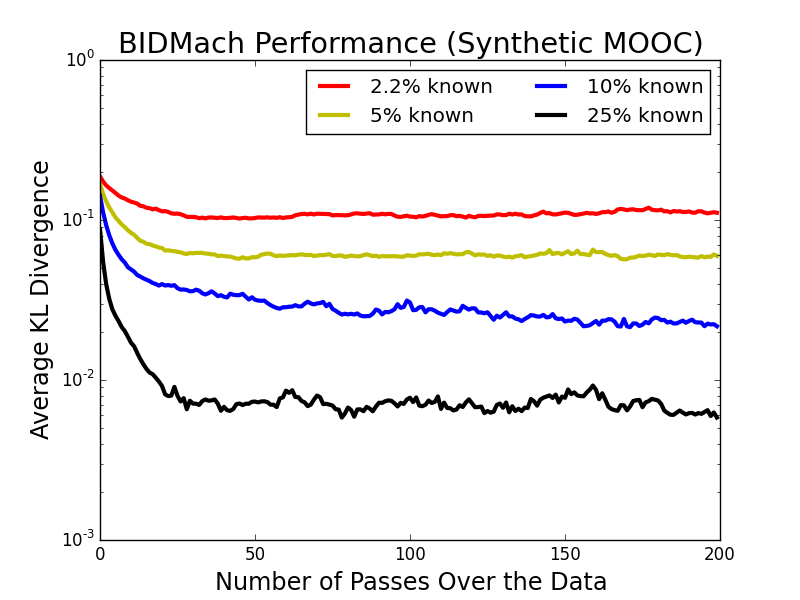
\includegraphics[width=1\textwidth]{fig_diff_sparsity_bidmach}
    \caption{Time and $KL_{\rm avg}$ (BIDMach).}
    \label{fig:kl_time_bidmach}
  \end{minipage}\hfill
    \begin{minipage}{.5\textwidth}
    \centering
    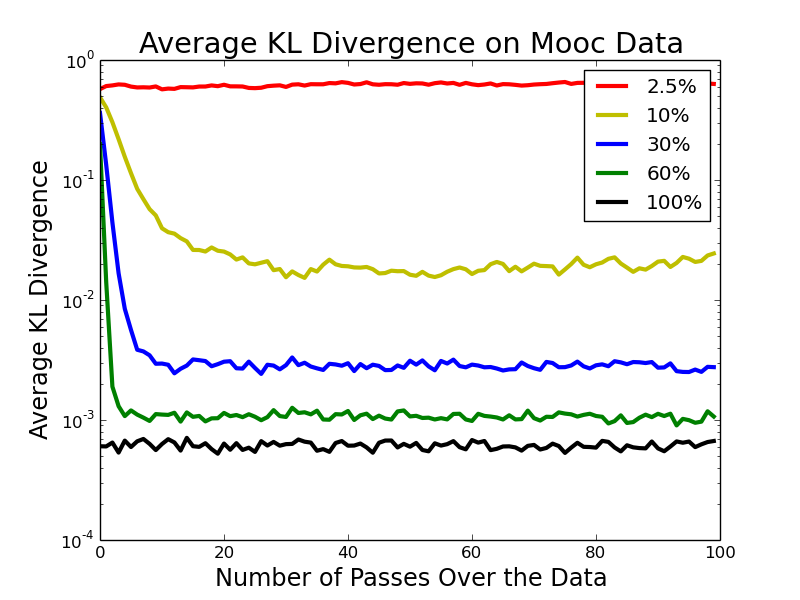
\includegraphics[width=1\textwidth]{fig_diff_sparsity_jags}
    \caption{Time and $KL_{\rm avg}$ (JAGS).}
    \label{fig:kl_time_jags}
  \end{minipage}
\end{figure}


% BIDMach (CPU) vs JAGS for the Real MOOC data *replicated*, with SAME=1.
% Batch size: we'll use 2184 (approx 4367/2) to be a fair comparision with previous table with
% Koller, because we usually like to have more than one mini-batch.
%
% Here are the BIDMach CPU (not GPU!) results on BITTER:
%
% Time=36.4890 secs, gflops=1.20 (1x)
% Time=71.5470 secs, gflops=1.22 (2x)
% Time=196.5920 secs, gflops=1.11 (5x)
% Time=387.2260 secs, gflops=1.13 (10x)
% Time=739.8330 secs, gflops=1.18 (20x)
% 
% Here are the CPU BIDMach times on STOUT with the same settings, which is what we report:
%
% Time=38.4290 secs, gflops=1.14 (1x)
% Time=75.0240 secs, gflops=1.17 (2x)
% Time=186.2360 secs, gflops=1.17 (5x)
% Time=358.4780 secs, gflops=1.22 (10x)
% Time=700.2980 secs, gflops=1.25 (20x)
% Time=1436.2930 secs, gflops=1.22 (40x)
%
% It takes a while with 20x, and absurdly long with 100x ... remember, the batch sizes are the same.
% Note: I suppose I should run this with 40% data as well...
%
% Notes on JAGS: we tried with 100x, but it crashed (ran out of memory) on stout, after almost 30
% minutes. And actually, 40% crashed as well. But on stout, BIDMach only uses 11.4% of the memory
% with 40% of the data.
\begin{table}[t]
\caption{BIDMach (CPU) vs. JAGS Runtime on (Replicated) Real MOOC Data}
\label{tab:bidmach_jags_realmooc}
\begin{center}
\begin{tabular}{ |c|c|c|c|c|c|c| } 
\hline
                       & 1x    & 2x     & 5x     & 10x    & 20x   & 40x   \\
\hline \hline
BIDMach Time(sec)/Iter & 0.182 & 0.375  & 0.931  & 1.792  & 3.501 & 7.181 \\ 
JAGS Time(sec)/Iter    & 4.876 & 13.745 & 29.150 & 94.075 &       & OOM   \\
\hline
\end{tabular}
\end{center}
\end{table}

We now benchmark our code on a Bayesian network with a nation-wide examination dataset from the
Dynamic Learning Maps (DLM) project\footnote{URL: \url{http://dynamiclearningmaps.org/}. There is no
official reference for this data.}. The data contains the assessment (correct or not) of student
responses to questions from the DLM Alternate Assessment System. After our preprocessing, there were
4367 students and 319 questions. From the DLM data source, each of the questions is considered to be
derived from a set of 15 basic concepts. We encode questions and concepts as variables and describe
their relationships with a Bayesian network from the DLM data.  Each question is considered an
``observed'' node in the Bayesian network, but with a very high missing value rate, as students only
got to answer a fraction of the questions.  Our data matrix, which has dimensions $(334\times
4367)$, ultimately ended up with a 2.2\% sparsity level.  Furthermore, the first 15 rows in the data
matrix are completely missing across all 4367 columns, since the 15 concepts are latent variables.
The inference task is to learn the CPTs of the Bayesian network from this extremely sparse data.

We evaluate our sampler on this MOOC data using two methods. The first involves running our sampler
on the original data until convergence. Then, we use the estimated set of CPTs and sample from that
via direct sampling to generate synthetic data, also of dimension $(334 \times 4367)$. We modify
that synthetic data matrix so that it also has a 2.2\% sparsity level and has missing data at the
same elements as the original data matrix. Then we re-run BIDMach on that data and test using the
same $KL_{\rm avg}$ metric from~(\ref{ssec:koller_data}), since we know the CPTs that ``generated''
the data.

Figure~\ref{fig:mooc_kl} plots the $KL_{\rm avg}$ for BIDMach with varying $m$ values. We ran the
sampler for several thousands of iterations but only show the first 300 for the sake of readability.
We see that, indeed, using $m=1$ as a reference, the Gibbs sampler appears to converge quickly to
the true distribution. It seems like the curve gets worse after the first 100 iterations, but
the long term trend (not shown here) is that it settles down at the same $KL_{\rm avg}$ from the 100
iteration point. It is also apparent from Figure~\ref{fig:mooc_kl} (and the long-term trend) that
$m=2$ and $m=5$ are better, showing that there is indeed a benefit to SAME with extremely sparse
data. What is interesting is that the performance of $m=10$ is \emph{worse} than $m=1$. Even after
thousands of iterations, the $m=10$ curve was essentially neck-to-neck with the $m=1$ curve, but
corresponds to a much slower runtime.

\textbf{Daniel: We are planning on including one JAGS curve ($m=1$) in Figure~\ref{fig:mooc_kl}. We
will need to explicitly state the runtimes for BIDMach/JAGS, probably just here in the text and not
in a figure/table. Also, I should explain the ``long term'' trend stuff better, perhaps even
extending the plot a bit. Finally, like before, I want to give an intuitive feel of the accuracy,
i.e., how many decimal points of accuracy?}

\begin{figure}[t]
  \centering
  \begin{minipage}{.5\textwidth}
    \centering
    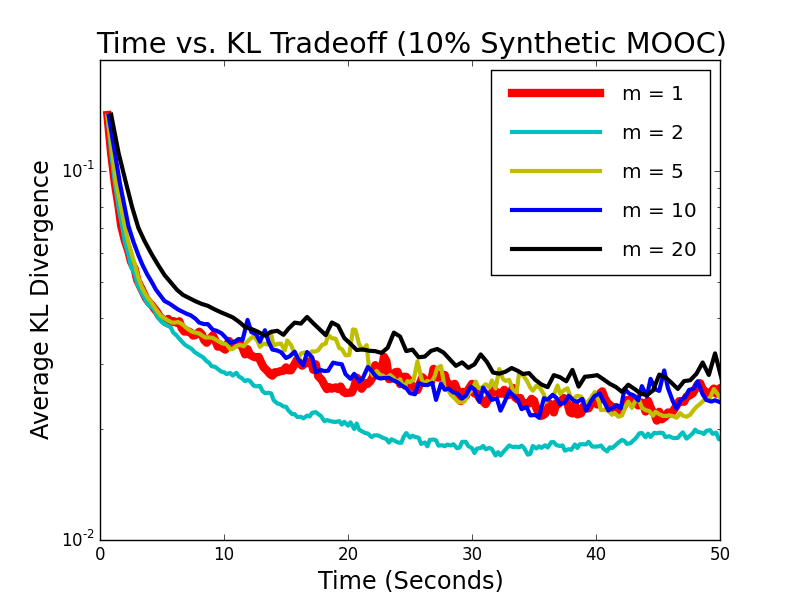
\includegraphics[width=1\textwidth]{fig_kltime_tradeoff_mooc}
    \caption{Time and $KL_{\rm avg}$ tradeoff.}
    \label{fig:mooc_kl}
  \end{minipage}\hfill
    \begin{minipage}{.5\textwidth}
    \centering
    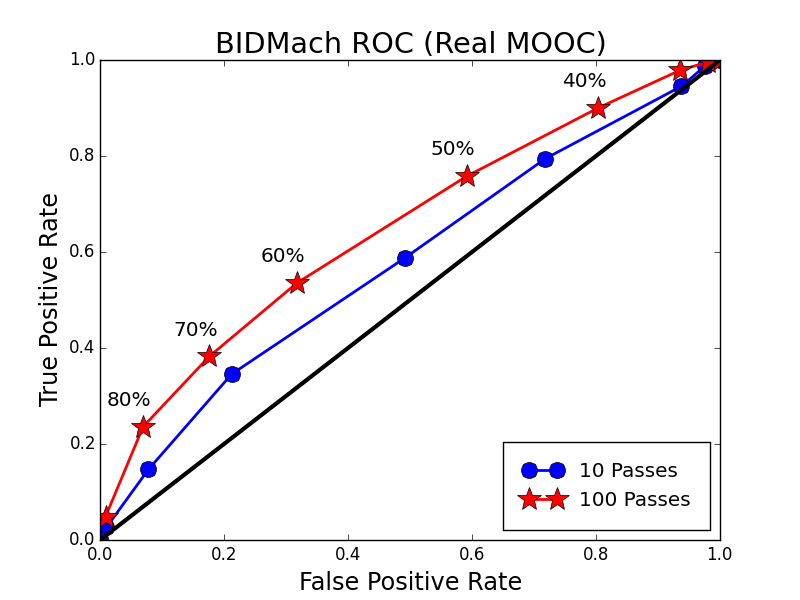
\includegraphics[width=1\textwidth]{fig_bidmach_real_mooc_roc_curve}
    \caption{MOOC data ROC curve.}
    \label{fig:mooc_accuracy}
  \end{minipage}
\end{figure}

The second way we evaluate our sampler is with prediction accuracy. We divide the original
data into a training and testing batch so that 80\% of the known data is in training. The training
set is for updating the CPTs. During the testing batch, we sample for 500 iterations using the
current CPTs (but \emph{without updating} them). For each of the known test points, we compute the
number of 0s and 1s sampled (from the 500 iterations), pick the majority to be our prediction,
and then compare it with the true value. Since only 2.2\% of the data is known, this is a challenging
prediction problem. Moreover, we divide the training and testing data into batches, so for each
student (i.e., column) in the test data matrix, we have no evidence.  Random guessing is equivalent
to 50\% accuracy since this is a binary prediction task.

We ran the prediction accuracy algorithm with SAME parameters $m=1$ and $m=5$ using three different
random seeds for each, to reduce the chances of one trial skewing the results.
Figure~\ref{fig:mooc_accuracy} plots the mean prediction accuracy (among three trials) for both SAME
parameters. Our sampler indeed learns to predict reasonably well and reaches roughly 61\% accuracy.
SAME is not beneficial in terms of accuracy or even the standard deviation of the accuracies (not
plotted here). This is likely because sampling 500 times to determine our prediction may cause
convergence to a result invariant to minor differences in CPTs.  Sampling only one time to determine
prediction accuracy resulted in about 56\% accuracy for $m=1$, and beyond 500 samples, we did not
observe improvements.

\subsection{Runtime vs. Throughput Tradeoff}\label{ssec:tradeoff}

% This should be in another section. We might consider splitting this in two if we have space. For
% both of these, I chose the largest batch size that we could do m = 50.
%
% Koller Data = (5 x 1,000,000)-dimensional, mini-batch size = 50,000, iterations = 200, seed = 777.
% This is with the sliding, rectangular window of samples, which is *slower* than the moving
% average,  hence we'll get slower gflops. Before, with complete truncation (but an incorrect
% graphical model, technically speaking) we were getting 13.90 for m = 50.
% Final statistics from BIDMach:
% Time=61.4750 secs, gflops=2.38 (m=1)
% Time=104.6140 secs, gflops=6.98 (m=5)
% Time=160.8270 secs, gflops=9.08 (m=10)
% Time=265.6820 secs, gflops=11.00 (m=20)
% Time=374.4060 secs, gflops=11.70 (m=30)
% Time=476.0510 secs, gflops=12.27 (m=40)
% Time=591.2360 secs, gflops=12.35 (m=50)
%
% MOOC Data = (334 x 43670)-dimensional, where we replicated the *real* mooc 5x column-wise. Hence,
% RM = Replicated MOOC. Again, this is with the sliding, rectangular window of samples. I was going
% to use 10x, but I would have had to shrink the batch size down to 100 (or even less than that), I
% think because putback requires extra memory or something. So I'm doing 5x, which lets me increase
% the batch size to 400. More advanced GPUs in the future will allow us to run this faster.

% Settings: mini-batch size = 400, SAME is the variable. 200 iterations and 777 seed as usual.
% Total runtimes were:
%
% Time=133.2460 secs, gflops=1.65 (m=1)
% Time=238.3670 secs, gflops=4.58 (m=5)
% Time=308.1950 secs, gflops=7.08 (m=10)
% Time=450.3450 secs, gflops=9.69 (m=20)
% Time=599.5060 secs, gflops=10.92 (m=30)
% Time=750.6940 secs, gflops=11.62 (m=40)
% Time=907.2790 secs, gflops=12.02 (m=50)
%
% Now for the actual table itself:
\begin{table}[t]
\caption{BIDMach (GPU) Runtime vs. GigaFlops on Large Data}
\label{tab:tradeoff}
\begin{center}
\begin{tabular}{ |c|c|c|c|c|c|c|c| } 
\hline
               & $m=1$ & $m=5$ & $m=10$ & $m=20$ & $m=30$ & $m=40$ & $m=50$  \\
\hline \hline
GigaFlops (K)  & 2.38  & 6.98  & 9.08   & 11.00  & 11.70  & 12.27  & 12.35   \\ 
Time/Iter (K)  & 0.307 & 0.523 & 0.804  & 1.328  & 1.872  & 2.380  & 2.957   \\
\hline 
GigaFlops (RM) & 1.65  & 4.58  & 7.08   & 9.69   & 10.92  & 11.62  & 12.02   \\ 
Time/Iter (RM) & 0.666 & 1.192 & 1.541  & 2.252  & 2.998  & 3.753  & 4.536   \\
\hline
\end{tabular}
\end{center}
\end{table}

We now discuss the impact of the SAME parameter in terms of runtime and throughput. We measure the
throughput and speed of our Gibbs sampler in terms of GigaFlops (gflops), a billion floating point
operations per second. It is possible to compute reasonable estimates of the maximum gflops
attainable for a computer. Therefore, in order for us to claim that the Gibbs sampler is as
optimized as it could be, we should argue that it attains gflops values that are close to the
theoretical limit, indicating that further improvement is unlikely beyond simply upgrading the
hardware.

\textbf{Daniel: We should compute the theoretical gflops limit.}

As the SAME parameter increases, it increases both the throughput (good) and runtime (bad) by
increasing the number of data points in our computations. The results from~\citep{SAME2015} suggest
that increasing $m$ for small values will increase throughput while not costing too much in runtime.
As one increases $m$ beyond a certain data-dependent value, then SAME ``saturates'' the algorithm
and results in stagnant throughput while significantly increasing runtime. It follows that a
reasonable objective for an experimenter is to run the Gibbs sampler on data with varying values of
$m$, and identify the point where further increases in $m$ start having an unfavorable runtime and
throughput tradeoff.

As an example, we used the Koller data from~(\ref{ssec:koller_data}), with 50\% of the data known
versus missing, but with \emph{one million} cases, beyond the feasible datasets of standard Gibbs
samplers. We ran the Gibbs sampler for 200 iterations on this data with a batch size of 50,000.
Table~\ref{tab:tradeoff} shows the time and gflops of the Gibbs sampler using different values of
$m$.  One can see that increasing $m$ for $m < 30$ results in steady gflops increases but
\emph{without} a substantial increase in time. Then SAME saturates the algorithm and the runtime
increases while the gflops stalls, reinforcing the conclusions from~\citep{SAME2015} and argues for
the importance of testing with a variety of $m$ values.

Notice that the runtimes listed are in seconds, and even with $m=50$, 200 iterations takes less than
10 minutes to complete --- we have barely scratched the limit of our sampler. In fact, one of the
main things that limits our sampler is the memory of GPUs, since we need to shrink the batch size
with large $m$. As memory on GPUs becomes cheaper, we will be able to run Gibbs sampling and perform
graphical model inference on larger datasets.


\section{Conclusions}\label{sec:conclusions}

We conclude that our Gibbs sampler is much faster than the state of the art (JAGS) in Gibbs sampling
and can be applied to data with several hundreds of variables. We also argue that SAME is beneficial
for Gibbs sampling, and that it should be the go-to method for researchers who wish to perform
inference on (discrete) Bayesian networks. Future work will explore the application of our sampler
to a wider class of real-world datasets.


\subsubsection*{Acknowledgments}

We thank Yang Gao, Biye Jiang, and Huasha Zhao for helpful discussions.

\bibliography{iclr2016_conference}
\bibliographystyle{iclr2016_conference}









%%% APPENDIX
%\clearpage
%\appendix
%
%\textbf{I expect that we will use eight pages for text, plus the ninth page for references. Then the
%remaining material (if any) will go here.}




% More stuff from Huasha:
%\subsection{Performance and Runtime}
%We first look at the efficiency of each system measured by giga floating point operations per second
%(Gflops). Intel VTune Amplifier is used to measure the flops numbers. As presented in Figure
%\ref{perf}, BIDMach achieves 5 Gflops and 1 Gflops for GPU and CPU respectively. The Gibbs sampler
%is bottlenecked by the calculation of sampling probability vectors which is implemented using SpMV
%operations. Such flops numbers are the hardware limit of SpMV operation. Jags and Infer.net operates
%at much lower flops rates. Note that the y-axis of the figure is in log-scale. The VTune profile
%results also show that Jags spend 70 \% of the runtime on disk IO, which is highly inefficient. We
%also observe that the memory usage of Infer.net is not efficient: on our PC with 8G memory, it
%cannot scale up to 10000 students (with the same statistics as the DLM pilot dataset we use).

\begin{comment}
% Daniel: I'm leaving this here for now, because this is some extra stuff from Huasha's old write-up
% that we might use.

We benchmark all the systems on fitting a Bayesian network with a nation-wide examination dataset
from the Dynamic Learning Maps (DLM) project. The dataset contains the assessment (correct or not)
of 30,000 students' responses to questions from the DLM Alternate Assessment System. There are 4000
students and 340 unique questions in the pilot experiment ,and the overall completion rate of the
questions is only 2.2 \% (assessment questions are tailored for each student). Each of the 340
questions is considered to be derived from a set of 15 basic concepts, and relations between
questions and concepts and within concepts are given. Each question is considered as a observed node
in the Bayesian network (with very high missing value rate), and each concept is considered as a
hidden node which never gets observed. Each node takes a binary value. The inference task is to
learn the parameter of the network on 80\% of the response assessment and predict on the rest 20\%
of the response. We use the prediction accuracy to measure the quality of the model. 

\subsection{Performance and Runtime}
We first look at the efficiency of each system measured by giga floating point operations per second
(Gflops). Intel VTune Amplifier is used to measure the flops numbers. As presented in Figure
\ref{perf}, BIDMach achieves 5 Gflops and 1 Gflops for GPU and CPU respectively. The Gibbs sampler
is bottlenecked by the calculation of sampling probability vectors which is implemented using SpMV
operations. Such flops numbers are the hardware limit of SpMV operation. Jags and Infer.net operates
at much lower flops rates. Note that the y-axis of the figure is in log-scale. The VTune profile
results also show that Jags spend 70 \% of the runtime on disk IO, which is highly inefficient. We
also observe that the memory usage of Infer.net is not efficient: on our PC with 8G memory, it
cannot scale up to 10000 students (with the same statistics as the DLM pilot dataset we use).

\begin{figure}[h!]
\centering
\includegraphics[scale = 0.7]{perf2.png}
\caption{Performance Comparison} 
\label{perf}
\end{figure}

Figure \ref{runtime2} shows the runtime until convergence for each inference engine. Again, time is
in log-scale. The Gibbs sample approach converges in about 200 iterations, while the EP algorithm
converges in 50 iterations. Infer.net is 3.5x faster than Jags. This is expected as symbolic method
is usually more efficient than sampling approach. BIDMach is 2-3 orders of magnitude faster than the
other systems. 

We can also verify that BIDMach is doing the same amount of work (floating point operations) as Jags
by multiplying the gflops number in Figure \ref{perf} with the run time in Figure \ref{runtime2}.

\begin{figure}[h!]
\centering
\includegraphics[scale = 0.7]{time2.png}
\caption{Runtime Comparison} 
\label{runtime2}
\end{figure}

\subsection{Prediction Accuracy}
For each node to be predicted, we sample 50 instances for that node from the learned network and
observed values, and then take the majority as the predicted value. The accuracy is measured as the
percentage of corrected predictions. A random guess will give an accuracy of 50\%. Figure
\ref{accuracy} shows the predicted accuracy as a function of number of iterations in training. Both
BIDMach and Jags achieves 65-67\% accuracy in around 200 iterations. However, BIDMach has a huge
advantage in terms of speed as shown in Figure \ref{runtime2}.

\begin{figure}[h!]
\centering
\includegraphics[scale = 0.7]{accuracy.png}
\caption{Accuracy Comparison} 
\label{accuracy}
\end{figure}

\end{comment}




\end{document}


%\section{Citations, figures, tables, references}
%\label{others}
%
%These instructions apply to everyone, regardless of the formatter being used.
%
%\subsection{Citations within the text}
%
%Citations within the text should be based on the {\tt natbib} package and include the authors' last
%names and year (with the ``et~al.'' construct for more than two authors). When the authors or the
%publication are included in the sentence, the citation should not be in parenthesis (as in ``See
%\citet{Hinton06} for more information.''). Otherwise, the citation should be in parenthesis (as in
%``Deep learning shows promise to make progress towards AI~\citep{Bengio+chapter2007}.'').
%
%The corresponding references are to be listed in alphabetical order of authors, in the
%\textsc{References} section. As to the format of the references themselves, any style is acceptable
%as long as it is used consistently.
%
%\subsection{Figures}
%
%All artwork must be neat, clean, and legible. Lines should be dark enough for purposes of
%reproduction; art work should not be hand-drawn. The figure number and caption always appear after
%the figure. Place one line space before the figure caption, and one line space after the figure. The
%figure caption is lower case (except for first word and proper nouns); figures are numbered
%consecutively.
%
%Make sure the figure caption does not get separated from the figure.  Leave sufficient space to
%avoid splitting the figure and figure caption.
%
%You may use color figures.  However, it is best for the figure captions and the paper body to make
%sense if the paper is printed either in black/white or in color.
%\begin{figure}[h]
%\begin{center}
%%\framebox[4.0in]{$\;$}
%\fbox{\rule[-.5cm]{0cm}{4cm} \rule[-.5cm]{4cm}{0cm}}
%\end{center}
%\caption{Sample figure caption.}
%\end{figure}
%
%\subsection{Tables}
%
%All tables must be centered, neat, clean and legible. Do not use hand-drawn tables. The table number
%and title always appear before the table. See Table~\ref{sample-table}.
%
%Place one line space before the table title, one line space after the table title, and one line
%space after the table. The table title must be lower case (except for first word and proper nouns);
%tables are numbered consecutively.
%
%\begin{table}[t]
%\caption{Sample table title}
%\label{sample-table}
%\begin{center}
%\begin{tabular}{ll}
%\multicolumn{1}{c}{\bf PART}  &\multicolumn{1}{c}{\bf DESCRIPTION}
%\\ \hline \\
%Dendrite         &Input terminal \\
%Axon             &Output terminal \\
%Soma             &Cell body (contains cell nucleus) \\
%\end{tabular}
%\end{center}
%\end{table}
%
%\section{Final instructions}
%Do not change any aspects of the formatting parameters in the style files.  In particular, do not
%modify the width or length of the rectangle the text should fit into, and do not change font sizes
%(except perhaps in the \textsc{References} section; see below). Please note that pages should be
%numbered.
%
%\section{Preparing PostScript or PDF files}
%
%Please prepare PostScript or PDF files with paper size ``US Letter'', and not, for example, ``A4''.
%The -t letter option on dvips will produce US Letter files.
%
%Consider directly generating PDF files using \verb+pdflatex+ (especially if you are a MiKTeX user).
%PDF figures must be substituted for EPS figures, however.
%
%Otherwise, please generate your PostScript and PDF files with the following commands:
%\begin{verbatim}
%dvips mypaper.dvi -t letter -Ppdf -G0 -o mypaper.ps
%ps2pdf mypaper.ps mypaper.pdf
%\end{verbatim}
%
%\subsection{Margins in LaTeX}
%
%Most of the margin problems come from figures positioned by hand using \verb+\special+ or other
%commands. We suggest using the command \verb+\includegraphics+ from the graphicx package. Always
%specify the figure width as a multiple of the line width as in the example below using .eps graphics
%\begin{verbatim}
%   \usepackage[dvips]{graphicx} ...
%   \includegraphics[width=0.8\linewidth]{myfile.eps}
%\end{verbatim}
%or % Apr 2009 addition
%\begin{verbatim}
%   \usepackage[pdftex]{graphicx} ...
%   \includegraphics[width=0.8\linewidth]{myfile.pdf}
%\end{verbatim}
%for .pdf graphics.  See section 4.4 in the graphics bundle documentation
%    (\url{http://www.ctan.org/tex-archive/macros/latex/required/graphics/grfguide.ps})
%
%A number of width problems arise when LaTeX cannot properly hyphenate a line. Please give LaTeX
%hyphenation hints using the \verb+\-+ command.
%
%\end{document}
